Let the crossover probability be $\alpha$.
Since the channel is symmetric,
\begin{align}\tag{1.0}
    \pr{1\ |\ 0} = \pr{0\ |\ 1} = \alpha = 0.1
\end{align}
\begin{figure}[h!]
    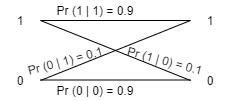
\includegraphics[width=\columnwidth]{solutions/ec/40/Code/Figure/Bin_Symm.png}
    \centering \caption*{Fig 1.0: Direct and Crossover Probability}
\end{figure}

Let a binomial r.v be X $\in$ $\{0, 1\}$ representing the number of bits transmitted incorrectly.
The sample space is given as $\{0, 1, 2, 3\}$.

\begin{equation}\tag{1.1}
    X \sim Bin(n=3, p=0.1)
\end{equation}
The binomial p.m.f. is given by:
\begin{equation}\tag{1.2}
    \pr{X=k} &= {n\choose k} p^{k} (1-p)^{n-k}\\
\end{equation}
Putting the values of X in (1.2) and sum up to get the probability of correct decoding,
\begin{equation}\tag{1.3}
    \begin{split}
        \pr{X=0} &= {3\choose 0} (0.1)^{0} (1-0.1)^{3-0}\\
                 &= (0.9)^{3}\\
        \pr{X=1} &= {3\choose 1} (0.1)^{1} (1-0.1)^{3-1}\\
                 &= 3\ (0.1)\ (0.9)^{2}
    \end{split}
\end{equation}
The probability of correct decoding is given by,
\begin{equation}\tag{1.4}
    \begin{split}
        P_c &= \pr{X=0} + \pr{X=1}\\
            &= (0.9)^{3} + 3\ (0.1)\ (0.9)^{2}\\
            &= 0.972\\
    \end{split}
\end{equation}
The average probability of error \\
\begin{equation}\tag{1.5}
    \begin{split}
            P_e  &= 1\ -\ P_c\\
                   &= 1\ -\ 0.972\\
                   &= 0.028
    \end{split}
\end{equation}
